Although the benchmark solutions utilized in the previous
subsections incorporate among others the leak-off term with a square root
singularity, there is no analytical solution for the Carter leak-off. In
\citet{Kovalyshen}, one can find the numerical results for such a case. This data may be utilized as a reference
solution. Unfortunately, the authors provide only some rough
estimation of the solution error. Surprisingly, they do not even
verify their numerical scheme against the early time asymptotic
model (considered as an analytical benchmark) to establish
quantitatively the accuracy of computations for the zero leak-off
case.

The numerical method used in \citet{Kovalyshen} is based on an
implicit finite volume algorithm. The data collected  in their Table 1 (p.332)
describes the normalized values of the crack length, the crack propagation speed and
the crack opening at $x=0$, at a number of times steps in the
interval $t\in [10^{-5},5\cdot 10^2]$. There is no precise
information on the utilized number of control volumes and the time
stepping strategies (the mentioned number of 10 control volumes
refers to the presented graphs, but it is not clear if the data from
table was obtained for the same parameters). The format of data
record (with five decimal digits) suggests that the guaranteed
solution accuracy is of the same level.


In the following we compare our numerical solution (see  Table \ref{table_Carter}) with that
by \citet{Kovalyshen}. Note that, due to different normalizations, our normalized  crack length, $L$, is two times greater than respective value in their paper. Our data was
obtained by the solver based on $U$ variable for $N=1000$ nodal points. Although
from the previous analysis it emerges that the system for $\Omega$
can provide better accuracy of $L$, we do not use it here to avoid an
additional postprocessing (numerical differentiation) when computing $w(0,t)$. On the other hand, in the light of previous
investigations, the system for $U$ for $N=1000$ can give the
accuracy of $L$ up to $10^{-6}$.


First, we present the graphs for evolution of the crack length, $L(t)$, -
Fig.~\ref{K_D_Lenght}, and the crack aperture at zero point, $w(t,0)$ - Fig.~\ref{K_D_w_0}. They depict the data for early time and
large time asymptotic models (respective formulae can be found also in
\citet{Kovalyshen}), and the numerical results
for a transient regime connecting these asymptotes. The solution by
\citet{Kovalyshen} is indicated by markers. A figure, equivalent to Fig.~\ref{K_D_Lenght}, has been also published in \citet{Nordgren}, however there is no data
available for comparison.

\begin{figure}[h!]
\center
    %\hspace{-2mm}
    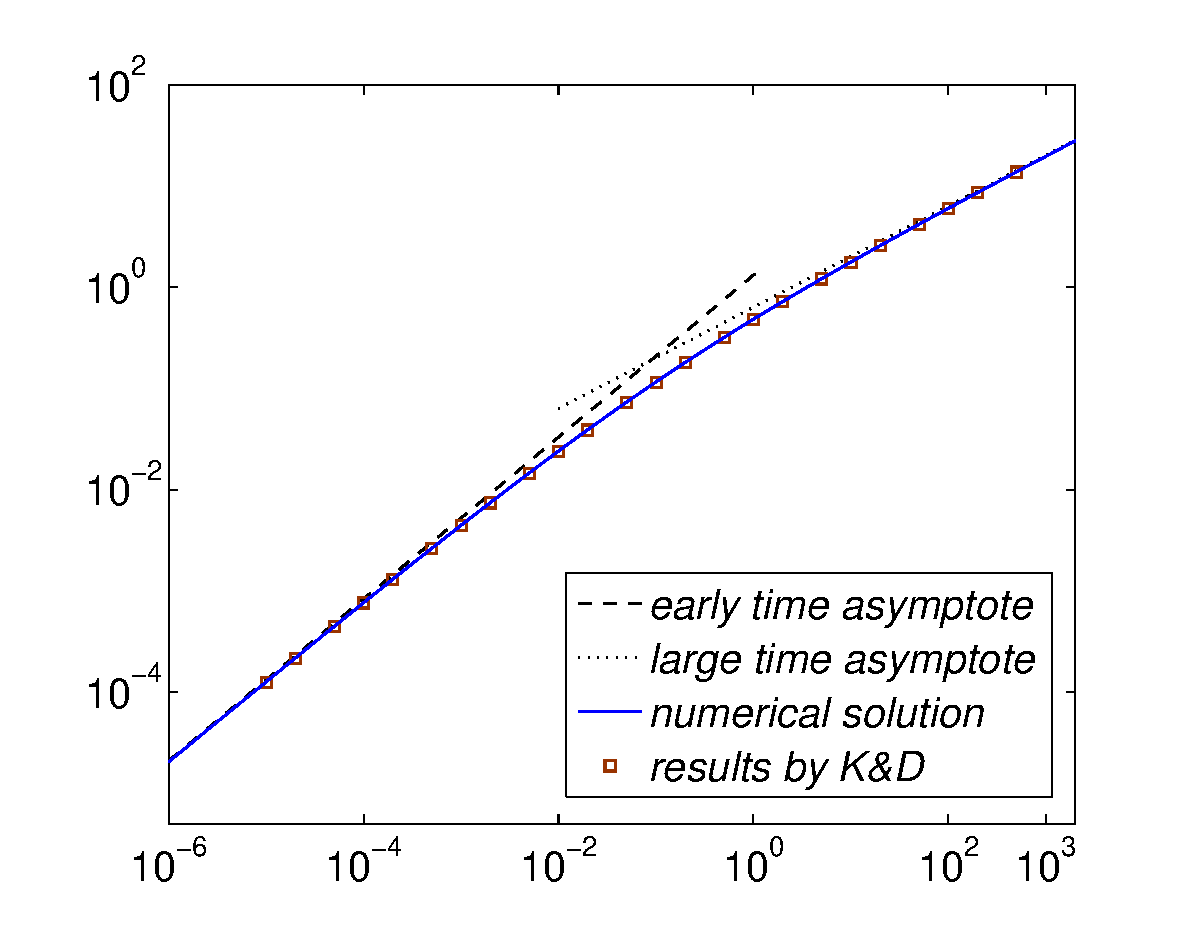
\includegraphics [scale=0.35]{3_PKN_numerical/vs_kov/K_D_Lenght.eps}
    \put(-100,-2){$t$}
    \put(-210,80){$L(t)$}


    \caption{The crack length evolution in time.}
\label{K_D_Lenght}
\end{figure}



We analyze the time interval $t \in[10^{-8},10^8]$ where the initial conditions
correspond to the early time asymptote for $t=10^{-8}$. The same
initial time was taken by \citet{Kovalyshen}, but the
authors presented their data starting from $t=10^{-5}$. In order to
increase the legibility of the graphs, we have truncated the time
axis to the range $t \in[10^{-6},5\cdot10^3]$, while the complete data
is presented in Table \ref{table_Carter}.


In Fig.~\ref{K_D_u} we show the normalized crack propagation speed, defined in a manner introduced by \citet{Kovalyshen}.


\begin{figure}[h!]
\center
    %\hspace{-2mm}
    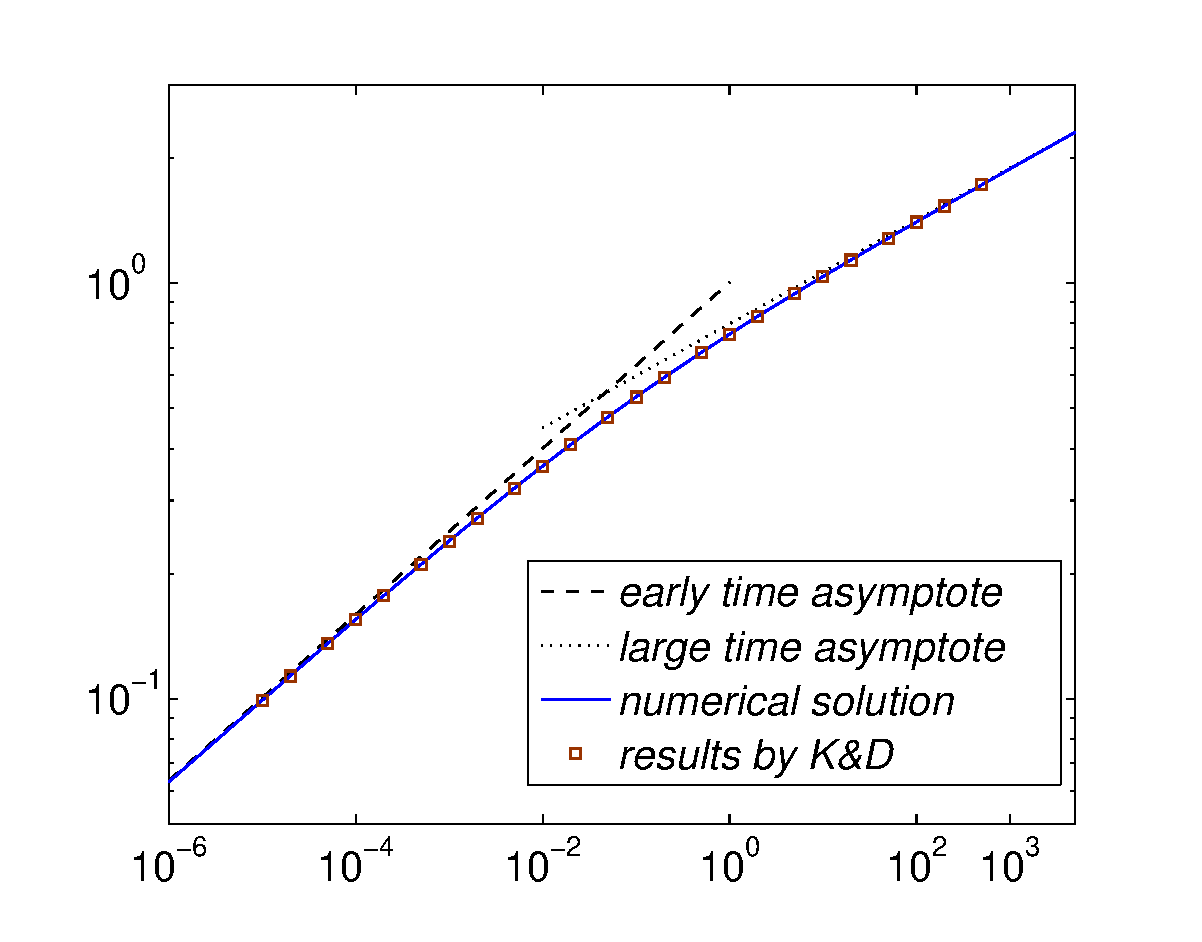
\includegraphics [scale=0.35]{3_PKN_numerical/vs_kov/w_0_symp.eps}
    \put(-100,-2){$t$}
    \put(-210,80){$w(t,0)$}

    \caption{The evolution of crack opening at zero point, $w(t,0)$.}
\label{K_D_w_0}
\end{figure}




\begin{figure}[h!]
\center
    %\hspace{-2mm}
    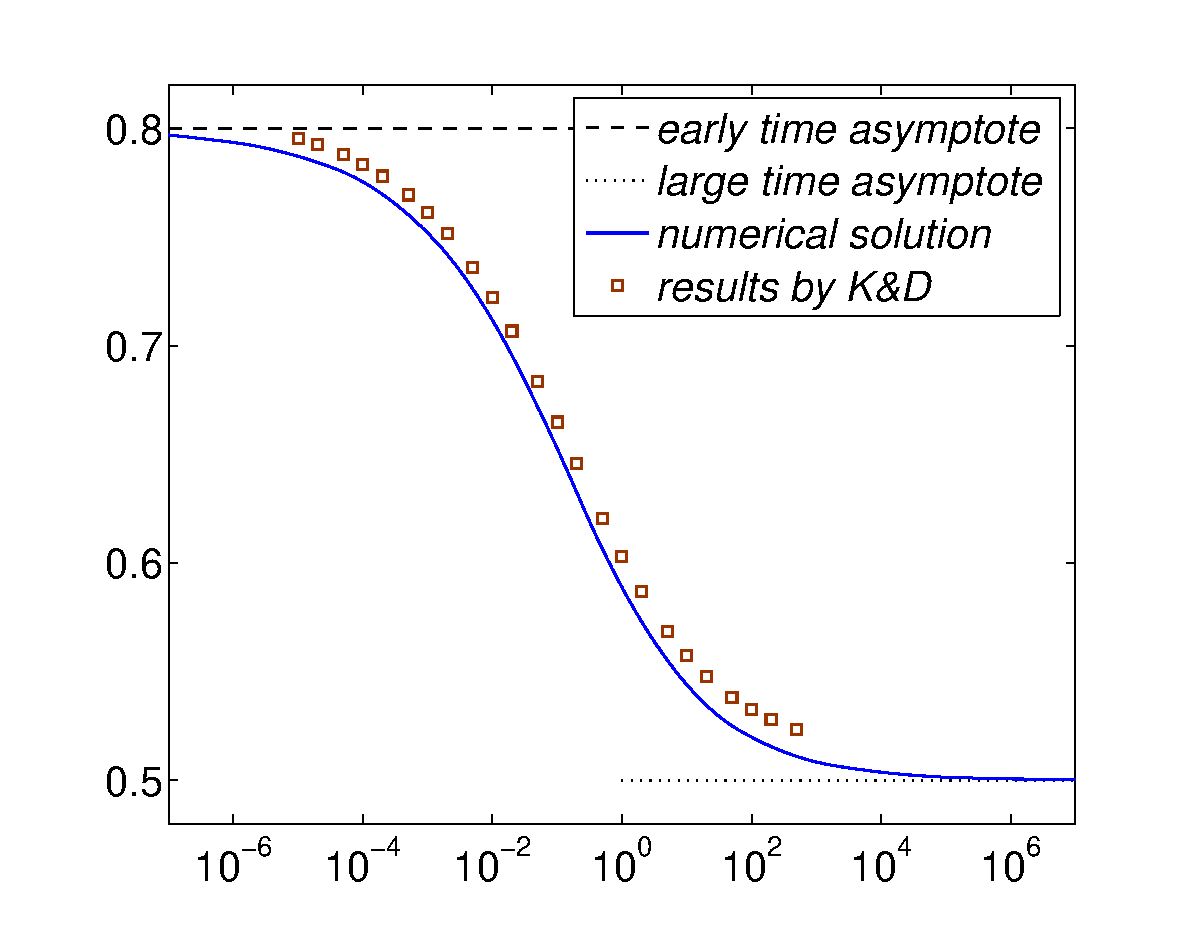
\includegraphics [scale=0.35]{3_PKN_numerical/vs_kov/u_asymp.eps}
    \put(-100,-2){$t$}
    \put(-205,80){$u(t)$}

    \caption{The evolution of the normalized crack propagation speed.}
\label{K_D_u}
\end{figure}


As can be seen in the Fig.~\ref{K_D_Lenght} -- Fig.~\ref{K_D_w_0}, in the presented scale, our solution is
undistinguishable from that by \citet{Kovalyshen} in terms of $L(t)$ and $w(t,0)$.
However, the normalized crack propagation speeds differ appreciably from each other. It shows that our solution
fit the asymptotes very well, which suggests its good quality. We cannot
examine, how the solution of \citet{Kovalyshen} approaches the asymptotic values due to the shortage of data for time intervals $t<10^{-5}$ and $t>5\cdot 10^3$ in their table.

In the analyzed case, the value of the parameter $Q_l(t)/q_0(t)$ changes continuously with time from zero to unit.
From the data presented in \citet{MWL} and in this paper, one can conclude that for $N=100$ nodal points, the relative error of the crack length
changes from $10^{-6}$ to $10^{-4}$ with the increase of the parameter $Q_l/q_0$.
On the other hand, analyzing the data from Fig.~\ref{fig:err_N_plots} -- Fig.~\ref{fig:err_N_plots_L} ($Q_l/q_0=0.9$), one can expect the achievable level
of accuracy of the order $10^{-7}$ for $N=1000$. This suggest that, in our computations, the relative error of $L$ varies between $10^{-4}$ and $10^{-6}$.

In order to additionally asses the credibility of our solution (computed for $N=1000$ and presented in the Table \ref{table_Carter}),
we show in Fig.~\ref{dev_L} the relative deviations between it and other solutions.
Namely, we analyze the crack lengths $L$ provided by: a) early and large time asymptotes;
b) the solution by \citet{Kovalyshen};
c) the solution obtained for 100 nodal points and d) the solution obtained for 1000 nodal points at another starting point $t_0=10^{-7}$.
\begin{figure}[h!]
\center
    %\hspace{-2mm}
    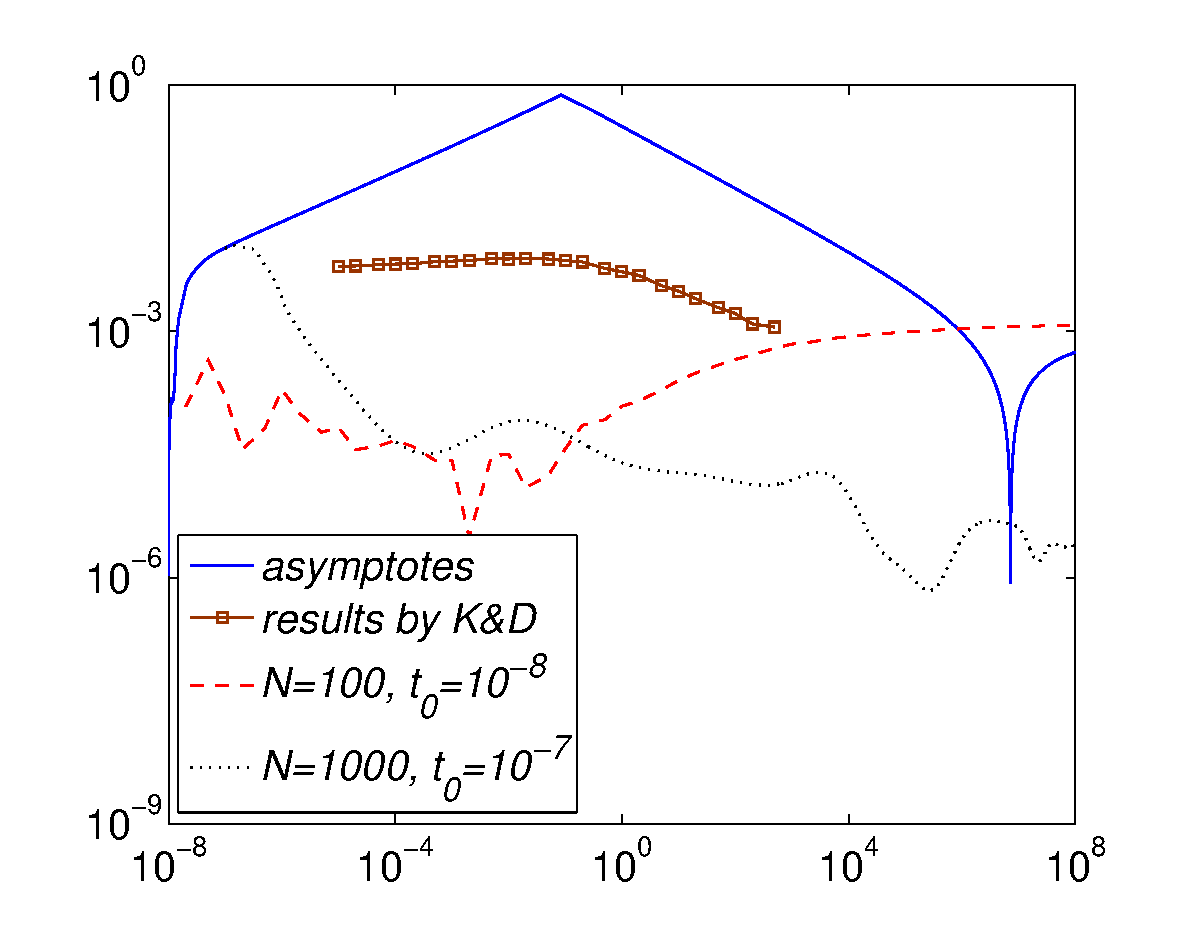
\includegraphics [scale=0.35]{3_PKN_numerical/vs_kov/dev_L.eps}
    \put(-100,-2){$t$}

    \caption{Relative deviations from the numerical solution for $L$.}
\label{dev_L}
\end{figure}


When tracing the data from Fig.~\ref{dev_L} we can see that the deviations of $L$ from the early and large time asymptotes at the ends of the considered interval are of the order $10^{-4}$. Moreover, the relative deviation of the solution obtained for 100 points is of the same order in almost entire  time range, which corresponds very well to the figures from Tab~\ref{table_very_bad_benchmark}. The discrepancy between the reference solution and the solution for $t_0=10^{-7}$ decreases rapidly with time. The last observation confirms the credibility of the reference solution.

We do not present respective graph for $w(t,0)$. However, it is worth mentioning that in this case the deviations from the asymptotes were even lower than for $L$, while the deviation of the solution for $N=100$ did not exceed the value of $10^{-4}$ on the substantial part of the interval.

The relative discrepancies between the components of our solution and the solution by \citet{Kovalyshen} are shown in Fig.~\ref{dev_Kov}. Here $d_L$, $d_{w(0,t)}$ and $d_u$ refer to the deviations of the crack length, $L$, the crack opening, $w(t,0)$ and the normalized crack velocity, $u$, respectively.


\begin{figure}[h!]
\center
    %\hspace{-2mm}
    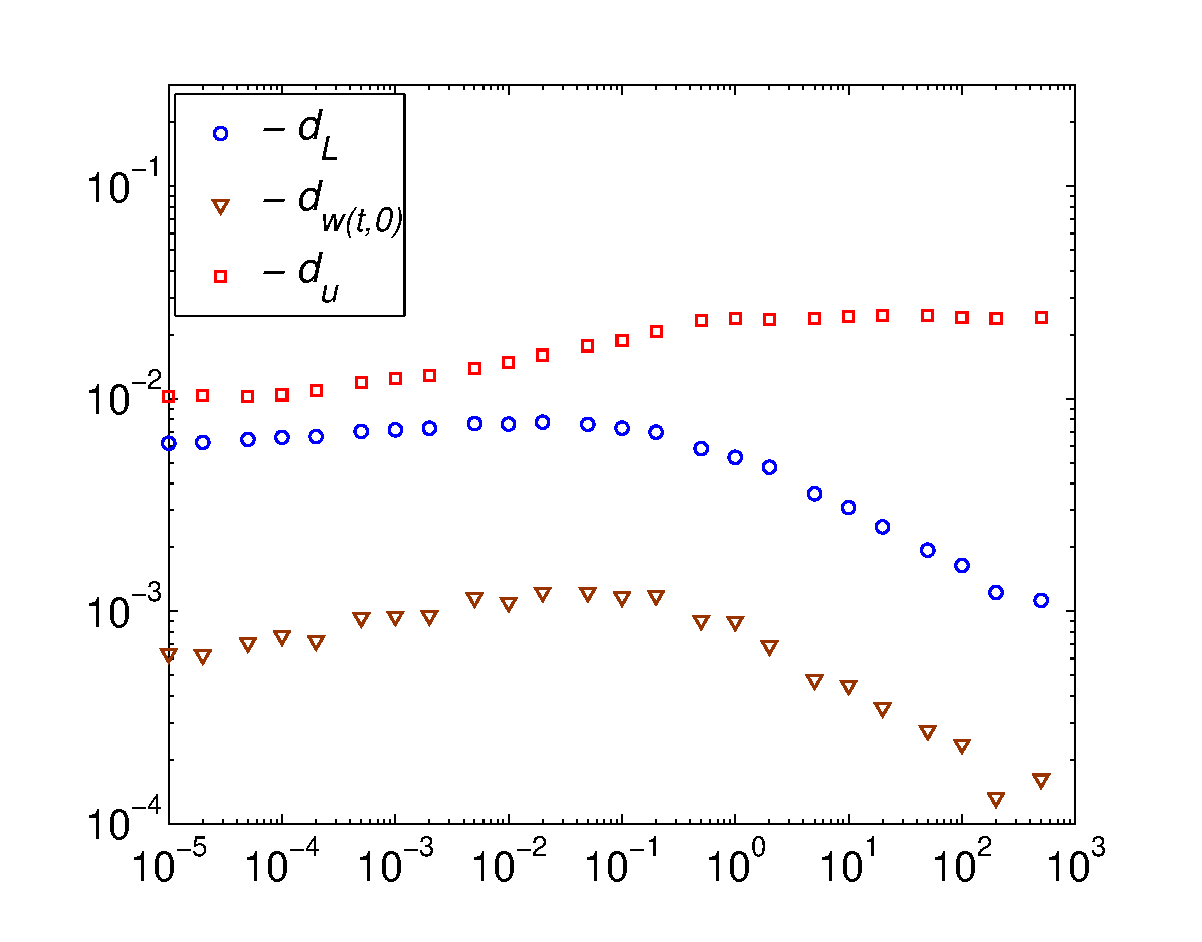
\includegraphics [scale=0.35]{3_PKN_numerical/vs_kov/Kov_odch.eps}
    \put(-100,-2){$t$}


    \caption{Relative deviations of the solution by \citet{Kovalyshen} from the results reported in Table \ref{table_Carter}.}
\label{dev_Kov}
\end{figure}

In the light of the presented results, we believe that the data collected in Table \ref{table_Carter} provide the accuracy  \textbf{at least} of the order $10^{-4}$ for both, the crack length, $L$, and the crack opening at $x=0$. Moreover, in the considerable time range ($10^{-6}< t<10^{6}$), one can expect the error lower by up to two orders of magnitude.
The normalized crack propagation speed $u$ is computed with accuracy of one to two orders of magnitude lower.

Summarizing the above discussions, the level of accuracy for the results tabulated by \citet{Kovalyshen} can be estimated as $10^{-3}\div 10^{-2}$ for $L$, $10^{-4} \div 10^{-3}$ for $w(t,0)$ and of the order $10^{-2}$ for $u$.

\begin{table}[H]
\centering
\begin{tabular}{c|c|c|c|c|c|c|c|c|c|}
\cline{1-4}
\multicolumn{1}{|c|}{$\log(t)$}&$L(t)$&$w(t,0)$&$u(t) \times 10$
\\ \cline{1-4}
\multicolumn{1}{|c|}{$-7$}&3.283747e-6&3.988347e-2&7.9701
 \\ \cline{1-4}
\multicolumn{1}{|c|}{$-6$}&2.049209e-5&6.298786e-2&7.9355
 \\ \cline{1-4}
\multicolumn{1}{|c|}{$-5$}& 1.265786e-4&9.915967e-2&7.8716
 \\ \cline{1-4}
\multicolumn{1}{|c|}{$-4$}& 7.660018e-4&1.551088e-1&7.7536
 \\ \cline{1-4}
\multicolumn{1}{|c|}{$-3$}&4.456291e-3&2.397462e-1&7.5185
 \\ \cline{1-4}
\multicolumn{1}{|c|}{$-2$}&2.412817e-2&3.629593e-1&7.1173
 \\ \cline{1-4}
\multicolumn{1}{|c|}{$-1$}&1.163591e-1&5.326638e-1&6.5267
 \\ \cline{1-4}
\multicolumn{1}{|c|}{$0$}&4.849863e-1&7.541837e-1&5.8885
 \\ \cline{1-4}
 \multicolumn{1}{|c|}{$1$}&1.779508e0&1.037495e0&5.4408
 \\ \cline{1-4}
 \multicolumn{1}{|c|}{$2$}&6.035529e0&1.403522e0&5.1993
 \\ \cline{1-4}
  \multicolumn{1}{|c|}{$3$}&1.968511e1&1.883411e0&5.0847
 \\ \cline{1-4}
  \multicolumn{1}{|c|}{$4$}&6.308563e1&2.518338e0&5.0378
 \\ \cline{1-4}
  \multicolumn{1}{|c|}{$5$}& 2.006370e2&3.362113e0&5.0146
 \\ \cline{1-4}
  \multicolumn{1}{|c|}{$6$}&6.360179e2&4.485636e0&5.0071
 \\ \cline{1-4}
  \multicolumn{1}{|c|}{$7$}&2.013373e3&5.982935e0&5.0029
 \\ \cline{1-4}
  \multicolumn{1}{|c|}{$8$}&6.369722e3&7.979082e0&5.0014
 \\ \cline{1-4}
\end{tabular}
\caption{Numerical solution of the PKN fracture.}
\label{table_Carter}
\end{table}